\chapter{Classification}

\epigraph{Classification is the act or process of dividing things into groups according to their type. }{\textit{Cambridge dictionary}}

Classification in machine learning involves assigning input data to a specific class label based on information learned from training data. An example of this is a bio-authentication system where a face is classified as either "authorized" or "rejected" based on pre-trained information. The concepts from regression methods, such as training and testing data sets, residuals or errors, cost function, and independent variables, also apply to classification.

In the project discussed in section \ref{sec:LRproject1}, the sale amount is predicted based on the advertising cost. As an illustration, consider a scenario where we want to determine whether a predicted sales amount meets a target or not. The output can only be two values: "meets the target" (yes) or "does not meet the target" (no). This is known as a \emph{binary classification} problem, as there are only two possible outputs: "yes" and "no".


Binary classification problems are commonly used in identifying specific outcomes based on the labelled data, such as:
\begin{itemize}
  \item Determining whether an email is spam (1) or not (0)
  \item Identifying if a tumor is malignant (1) or benign (0)
  \item Predicting if a customer will default on a loan (1) or not (0) based on their behavior.
\end{itemize}


A \textbf{multi-class classification} problem involves assigning an input to one of more than two possible classes. For example, consider a task of labeling names from 135 different races in Myanmar, where the goal is to classify each name into one of the 135 races.

Another type of classification problem is called \textbf{multi-label classification}, where an input can be assigned to multiple classes. This type of problem is commonly found in text categorization, where a text document may belong to multiple labels or categories.

\newpage
\section{Performance Evaluation}\label{sec:Clsevaluation}

This section discusses the most commonly used metrics for evaluating the performance of a classification model, specifically in the context of binary classification problems. These metrics include measures such as accuracy, precision, recall, F1 score, and ROC-AUC. It is important to note that there is no one-size-fit-all metric to measure the performance of a classification model.

Each of these metrics has its own unique characteristics and is better suited for certain types of classification problems. For example, accuracy is a good metric when the classes are balanced, but precision and recall are more appropriate when the classes are imbalanced. Additionally, the ROC-AUC metric is widely used for evaluating the performance of models that predict probabilities. The appropriate metric to be used will depend on the specific problem at hand and context.

The metrics used to evaluate performance in binary classification problems can be applied to multi-class classification problems by calculating them for each class and then taking the average.

\subsection{Confusion Matrix}
In binary classification problem, there are only two possible outputs: one and zero.
\begin{table}[!ht]
\centering
\begin{tabular}{|c|c|c|c|c|c|c| }
    \hline
    Predicted output & 0 & 1 & 0 & 0 & 1 & 1  \\
    \hline
    Actual Label & 0 & 0 & 1 & 0 & 0 & 1\\
    \hline
\end{tabular}
\caption{Example labels of predicted and actual output.}\label{tb:cmTable}
\end{table}

Table \ref{tb:cmTable} illustrates examples of predicted outputs and actual labels, with four possible combinations:
\begin{itemize}
  \item Case 1: Predicted as one and actual value is one (11)
  \item Case 2: Predicted as one but actual value is zero (10)
  \item Case 3: Predicted as zero and actual value is one  (01)
  \item Case 4: Predicted as zero and actual value is zero (00)
\end{itemize}

A successful classification model will have a higher ratio of cases 1 and 4 and a lower ratio of cases 2 and 3. Table \ref{tb:cmTable} illustrates that there are 1 number of case 1 (11), 2 number of case 2 (10), 1 number of case 3 (01) and 2 number of case 4 (00). This information can be summarized in a square matrix form below:

\begin{figure}[!h]
  \centering
  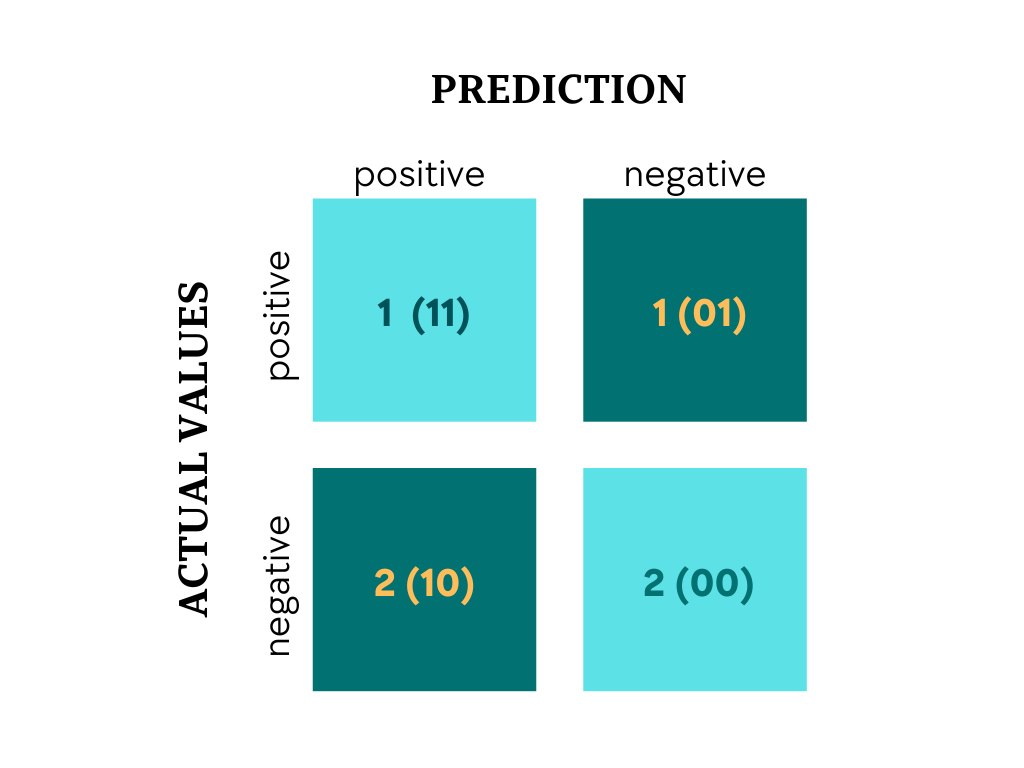
\includegraphics[width=9 cm]{CM_eg.png}
  \caption{Confusion Matrix for Table \ref{tb:cmTable}}
  \label{fig:cm_eg}
\end{figure}

The first column represents the instances where the model predicted a positive outcome. Out of the 3 instances where the model predicted positive, one was correct as the actual value was also positive. This is reflected in the top-left box. The remaining 2 instances were incorrect predictions, as the actual value was negative, and this is reflected in the bottom-left box.

The second column represents the instances where the model predicted a negative outcome. Out of the 3 instances where the model predicted negative, two were correct as the actual values were also negative. This is reflected in the bottom-right box. The remaining one was an incorrect prediction, as the actual value was positive, and this is reflected in the top-right box.

\begin{figure}[!h]
  \centering
  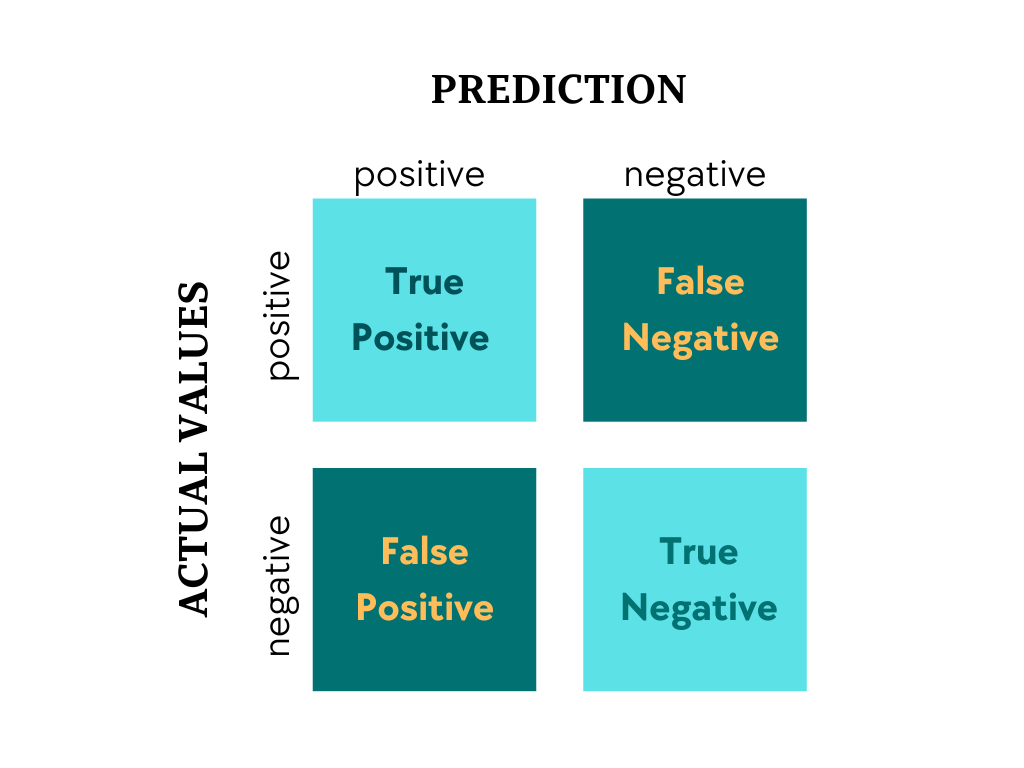
\includegraphics[width=8 cm]{Classifier_CM.png}
  \caption{Confusion Matrix: rows (Actual) and columns (Prediction)}
  \label{fig:cls_cm}
\end{figure}

In general, a \textbf{confusion matrix} is a table that summarizes the performance of a classification model by comparing predicted values with actual values. (Refer to Figure \ref{fig:cls_cm}.) It typically has four quadrants, each representing one of the following outcomes:

\begin{itemize}
  \item True Positive (\textbf{TP}) refers to instances where the model predicted a positive outcome and the actual value was also positive.
  \item False Positive (\textbf{FP}) refers to instances where the model predicted a positive outcome but the actual value was negative.
  \item False Negative (\textbf{FN}) refers to instances where the model predicted a negative outcome but the actual value was positive.
  \item True Negative (\textbf{TN}) refers to instances where the model predicted a negative outcome and the actual value was also negative.
\end{itemize}

In this book, we align with the convention used in the Python sklearn library where the rows of the confusion matrix represent the actual values and the columns represent the predicted values. However, it is worth noting that there is another common format of the confusion matrix where the rows represent the predicted values and the columns represent the actual values.

\subsection{Accuracy}
Accuracy is a metric that quantifies the proportion of correct predictions made by a model. Using the example in Table 3.1, there are six predictions made and three of them are correct, the accuracy of the model is 50\%. Mathematically, the formula for calculating accuracy is defined as:

\begin{equation}\label{eqn_acc}
  Accuracy = \frac{TP + TN}{TP+FP+FN+TN}
\end{equation}

However, accuracy is not always an appropriate metric to evaluate the performance of a model when the classes are imbalanced. For example, let's consider a scenario where there are 15 positive cases and 85 negative cases.
\begin{figure}[!h]
  \centering
    \begin{subfigure}[b]{0.7\textwidth}
         \centering
         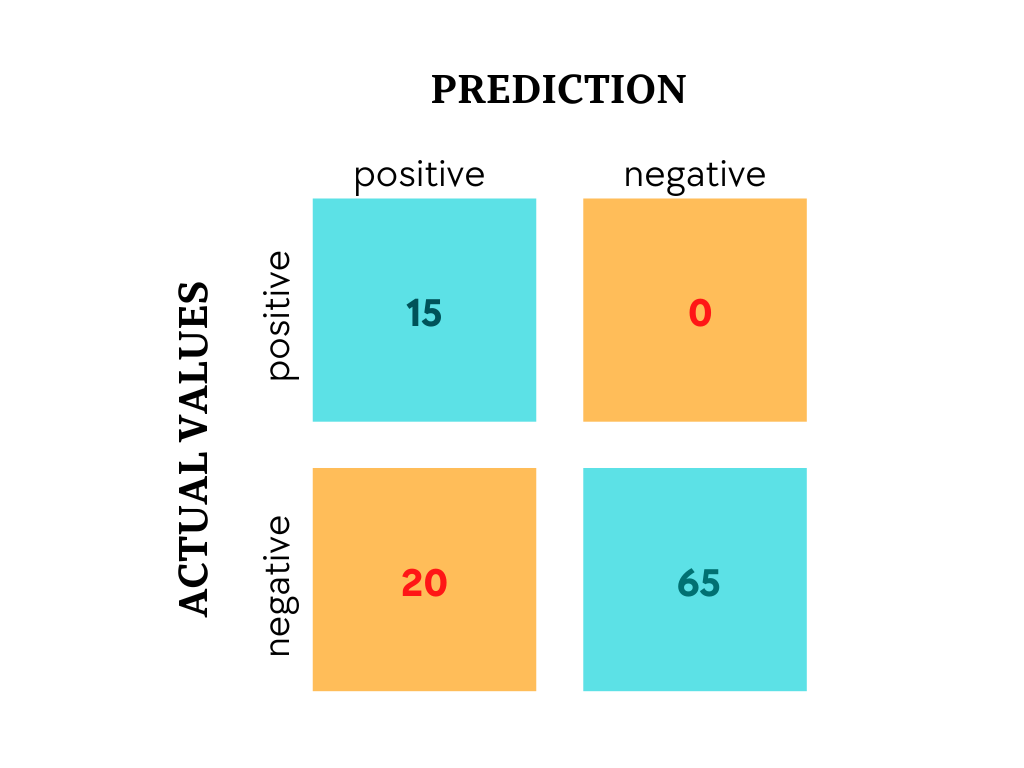
\includegraphics[width=5 cm]{cm_3e.png}
         \caption{Model 1}
         \label{fig:mdoel1_cm}
     \end{subfigure}
     \begin{subfigure}[b]{0.7\textwidth}
         \centering
         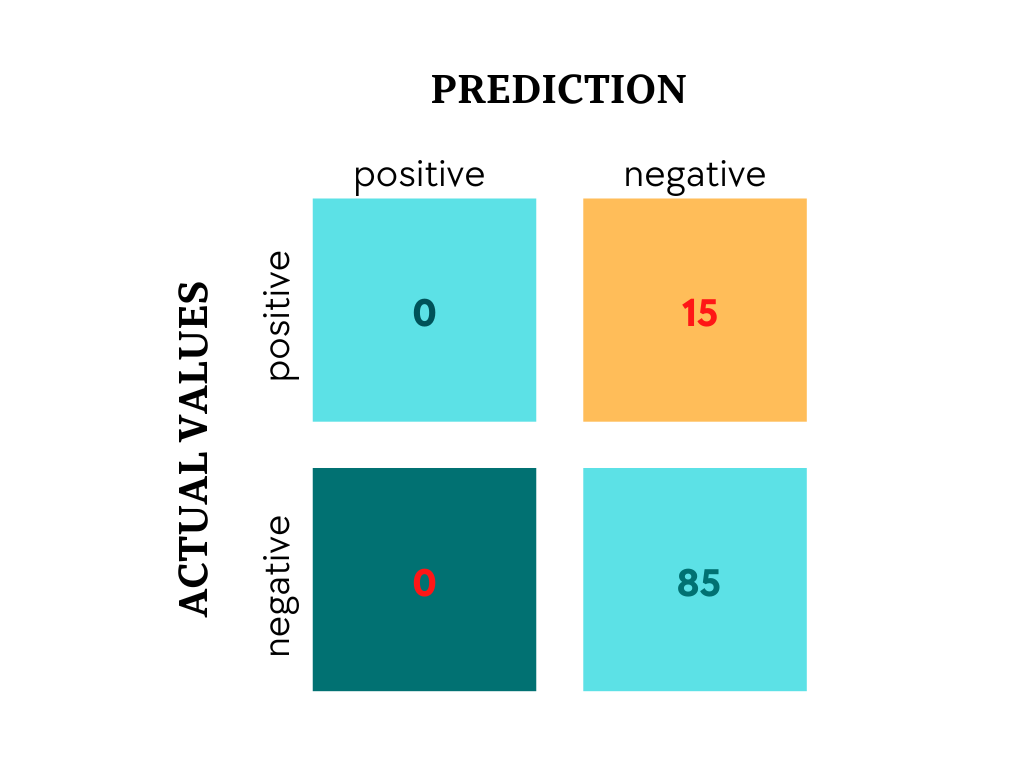
\includegraphics[width=5 cm]{cm_4e.png}
         \caption{Model 2}
         \label{fig:mdoel2_cm}
     \end{subfigure}
  \caption{Confusion Matrix from Model 1 and Model 2}
  \label{fig:cls_cm_Imb}
\end{figure} The confusion matrices for Model 1 and Model 2 are shown in Figure \ref{fig:cls_cm_Imb}. From the confusion matrices, it can be seen that Model 1 (Refer to Figure \ref{fig:mdoel1_cm}) has only $80\%$ accuracy and Model 2 (Refer to Figure \ref{fig:mdoel1_cm}) has $85\%$ accuracy. However, if we examine the confusion matrices carefully, Model 1 accurately predicts all positive cases and $76\%$ of the negative cases (75 out of 85), while Model 2 (Refer to Figure \ref{fig:mdoel2_cm}) did not detect any of the positive cases. If these models are developed for cancer detection, Model 2 is missing all the cancer patients.

In such scenarios, other metrics such as precision and recall should be considered.

\subsection{Precision}
Precision measures the proportion of true positive predictions out of all positive predictions made by a model and it is calculated as:
\begin{equation}\label{eqn_prec}
  Precision = \frac{TP}{TP+FP}
\end{equation}Precision is particularly important when minimizing false positives is a higher priority than minimizing false negatives. For example, in the case of a spam filter, it is more important to avoid marking a legitimate email as spam (false positive) than to allow a spam email to reach the inbox (false negative). High precision is therefore critical in problem like spam filtering systems.

\subsection{Recall (Sensitivity)}
Recall, also know as sensitivity or true positive rate, measures the proportion of actual positive cases that were correctly identified by the model and it is calculated as:
\begin{equation}\label{eqn_recall}
  Recall (\text{sensitivity}) = \frac{TP}{TP+FN}
\end{equation}Recall is particularly important in cases where missing a positive case (false negative) is more detrimental than having false alarms (false positives). This is often the case in medical applications such as cancer detection, where missing a cancer case is more dangerous than detecting one in a non-cancer patient. In such scenarios, recall should be as high as possible.

%Recall is also known as sensitivity, as it measures how well a model can detect positive cases and true positive rate, as it is calculated by dividing the number of accurately detected positive cases by the total number of actual positive cases.
%\newpage
\subsection{True Negative Rate (Specificity)}
The specificity, also known as the true negative rate, measures how many negative cases are accurately detected by the model. It is calculated as::
\begin{equation}\label{eqn_specificity}
  TNR (\text{Specificity}) = \frac{TN}{FP+TN}
\end{equation} Specificity is particularly useful when the cost of a false positive (predicting a negative case as positive) is high. An example of this can be a medical test for a rare disease. In this case, a false positive would mean that a healthy person is incorrectly diagnosed as having the disease, which would have severe consequences. In such scenarios, a high specificity is desired.

\subsection{F-score}
F-score, also known as F1-score, is a metric that combines both precision and recall into a single score, it is defined as:
\begin{equation}\label{eqn_Fscore}
  F-score = \frac{2*Recall*Precision}{Recall+Precision}
\end{equation}The F-score is high when both precision and recall are high, and low when either one of them has a low value. It is particularly effective in problems where both false positives and false negatives are considered equally important.
\newpage
\subsection{Area under the ROC (AUROC or AUC)}
The area under the ROC (receiver operating characteristic) curve is a widely used evaluation metric that measures a model's ability to distinguish between classes. It is calculated as the area under the Receiver Operating Characteristic (ROC) curve and AUC ranges between 0 and 1, with a value of 1 indicating a perfect classifier and a value of 0.5 indicating a classifier that is no better than random guessing.

AUC is commonly used to evaluate the performance of a model when the proportion of positive and negative cases is imbalanced. A high AUC value indicates that the model is able to correctly classify a large proportion of positive cases while also correctly classifying a large proportion of negative cases.

\noindent To understand AUC, it is important to first understand the ROC curve which plots two metrics:
\begin{itemize}
  \item True Positive Rate (TPR, also known as recall)
  \item False Positive Rate (FPR, which is 1 - specificity)
\end{itemize}

Many classification methods, such as logistic regression, produce a probability of an input belonging to the positive class. The class label is then obtained by comparing the resulting probability with a pre-defined threshold. A higher threshold value will reduce the number of positive predictions (both TP and FP).

\begin{table}[!h]
\centering
\begin{tabular}{|c|c|c|c|c|}
  \hline
  Threshold & TP & TN & TPR & FPR \\
  \hline
  0   & 117 & 0 & 1 & 1 \\
  \hline
  0.2 & 101 & 7013 & 0.863 & 0.001 \\
  \hline
  0.5(default) & 93 & 7037 & 0.795 & 0.0007 \\
  \hline
  0.8 & 93 & 7039 & 0.752 & 0.0004 \\
  \hline
  1 & 0 & 7042 & 0 & 0 \\
  \hline
\end{tabular}
\caption{Trade-off between TPR and FPR.}\label{tb:roc}
\end{table}

\begin{figure}[!h]
  \centering
  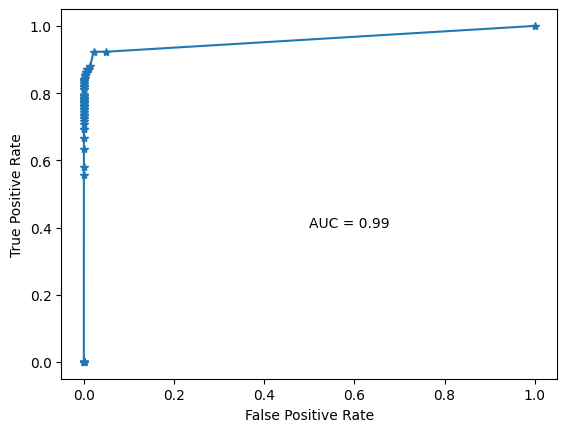
\includegraphics[width=7.5 cm]{auc.png}
  \caption{Binary ROC curve}
  \label{fig:auc}
\end{figure}

This is demonstrated in Table \ref{tb:roc}. There are $117$ actual positive cases (FN + TP) and $7042$ negative cases (TN + FP). When the threshold value is set to zero, all predictions are classified as positive cases, resulting in all positive cases correctly classified (TP = 117), and the true positive rate TPR is 1. As the threshold value increases, the true positive will decrease but the true negative will increase.

At the other extreme case, when the threshold value is set to 1, all cases are predicted as negative class, resulting in all negative cases correctly classified (TN = 7042) but none of the positive classes will be detected.

The ROC curve plots the true positive rate against the false positive rate, as shown in Figure \ref{fig:auc}. The AUC is computed by measuring the area under this curve. In this example, the model has a high AUC score of 0.99, indicating that it has a strong ability to accurately identify both positive and negative cases.


\newpage

\section{Logistic Regression}

Logistic regression maps input values to estimated target classes. It uses a sigmoid function, also known as the logistic function, to make predictions. Mathematically, it is defined as:
\begin{equation}\label{eq:ypredLR}
   \tilde{y} = g(\theta^T x) = \frac{1}{1+\exp(-\theta^T x)},
\end{equation}where $\theta$ is the model parameters and $x$ denotes an independent variable. In the case of a single feature, $\theta^T x$ is equal to $\omega_1 x + b$. The predicted values of $\tilde{y}$ can be interpreted as the probability of the target belong to the class 1 (or positive case) and it will always be between $0$ and $1$. This can be further illustrated by plotting the $g(z)$:

\begin{equation}\label{eq:ypredLR_z}
   g(z) = \frac{1}{1+\exp(-z)},
\end{equation} where $z$ is defined as $z = \theta^T x$.

Figure \ref{fig:sigmoid} illustrates that the output of the sigmoid function (g(z)) is always limited between 0 and 1. When the input value ($z$) approaches infinity, the output ($g(z)$) approaches 0 and when the input value ($z$) approaches negative infinity, the output ($g(z)$) approaches 1.  The predicted outputs (class labels) are obtained by applying a threshold value to the output of the sigmoid function $\tilde{y}$. The threshold value is usually set at 0.5 to classify the class label as either 0 or 1.

\begin{figure}[!h]
  \centering
  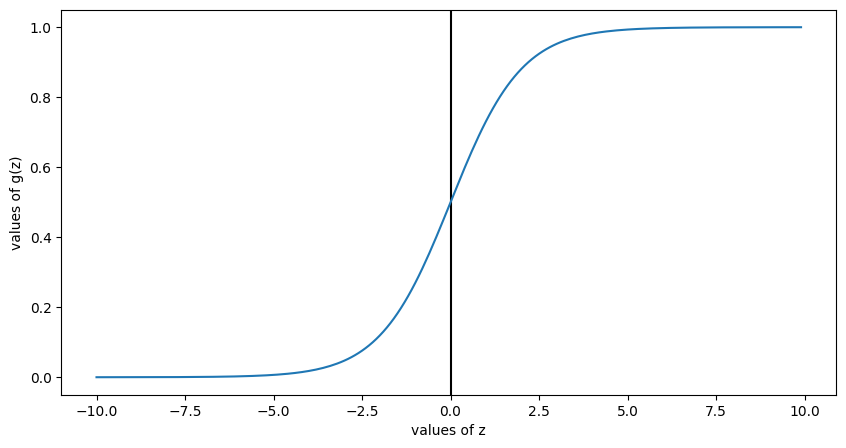
\includegraphics[width=8 cm]{demo_LR.png}
  \caption{Demonstration of Sigmoid Function}
  \label{fig:sigmoid}
\end{figure}

Since the target variable ($y$) in a binary classification problem is a categorical value that can only be 0 or 1, the cost function in logistic regression utilizes this property to predict the target class and the cost is defined as:
\begin{equation}\label{eqn:cost_LogR}
  J(\theta) = cost(g(z), y_i) = \begin{cases}
                    -\log (g(z)) &     \text{if $y_i = 1$}\\
                                 & \\
                    -\log (1-g(z)) &  \text{if $y_i = 0$}
                    \end{cases}
\end{equation} The above equation can be combined into a single equation as:
\begin{equation}\label{eqn:cost_LogR2}
  J(\theta) = -y_i \log (g(z)) - (1-y_i) * \log (1-g(z))
\end{equation}


If the estimated label $g(z)$ is the same with the actual output $y$, the cost value will be zero as shown in Table \ref{tb:LRcostR}.
\begin{table}[!ht]
\centering
\begin{tabular}{|c|c|r|}
  \hline
  Actual  & Estimated label & cost \\
  \hline
  & & $J(\theta) = -\log (g(z))$\\
  \hline
  $y =1$ & $g(z)=1$ & $J(\theta) = -\log (1)=0$\\
  $y =1$ & $g(z)=0$ & $J(\theta) = -\log (0)=1$\\
  \hline
  & & $J(\theta) = -\log (1-g(z))$\\
  \hline
  $y =0$ & $g(z)=1$ & $J(\theta) = -\log (1-1)=-1$\\
  $y =0$ & $g(z)=0$ & $J(\theta) = -\log (1-0)=0$\\
  \hline
\end{tabular}
\caption{Results of Cost function in \ref{eqn:cost_LogR}.}\label{tb:LRcostR}
\end{table}


In general, for multiple number of observations, the cost function can be defined as an average of the cost values for all observations.
\begin{equation}\label{eqn:cost_LogR_F}
  J(\theta) = -\frac{1}{N} \sum_{i=1}^N \left[y_i*log (g(z) + (1-y_i)*log(1-g(z)\right]
\end{equation} where $N$ is the number of data points (sample or observations). We can use an optimization algorithm, such as the gradient descent method discussed in section \ref{sec:GDS}, to find the best parameter $\theta$ that minimizes the cost.


\newpage

\subsection{Logistic Regression in Python}

The following code demonstrates the implementation of a logistic regression classifier using Python's sklearn library. The same steps outlined in section \ref{sec:model} are also applied in this example.

The 'fraud' data set \cite{web:fraudData} is used to predict whether a borrower will default or not, where default is defined as the borrower failing to make required payments on a debt. There are 30 features in the data set, with the target variable (default or non-default) listed in the 'Class' column. The remaining 29 columns are used as independent features.

\begin{lstlisting}[language=Python]
# ==================================================#
import pandas as pd

df=pd.read_csv('..\\data\\fraud.csv')
y = df['Class'].values
X = df.drop(columns = 'Class').values

from sklearn.model_selection import train_test_split

X_train, X_test, y_train, y_test = train_test_split(X,y,
                                    test_size = 0.33,
                                    random_state=1)

#--------------------------------------------------
## Using piepline to implement Logistic regression ##
#--------------------------------------------------
from sklearn.preprocessing import StandardScaler
from sklearn.linear_model import LogisticRegression
from sklearn.pipeline import Pipeline

steps = [('scaler', StandardScaler()),
         ('logReg', LogisticRegression())]

clf_pipeline = Pipeline(steps)
clf_pipeline.fit(X_train, y_train)
#--------------------------------------------------
## Model Evaluation ##
#--------------------------------------------------
from sklearn.metrics import classification_report
from sklearn.metrics import confusion_matrix
from sklearn.metrics import roc_auc_score

ypred_test = clf_pipeline.predict(X_test)
mat_clf = confusion_matrix(y_test, ypred_test)
report_clf = classification_report(y_test, ypred_test)

ypred_testP = clf_pipeline.predict_proba(X_test)
auc = roc_auc_score(y_test, ypred_testP[:,1])
# ==================================================#
\end{lstlisting}

\subsection{Hyper-parameters}
There are several optimization algorithms that can be used to solve the optimization problem in logistic regression, such as Newton method and Stochastic Average Gradient (SAG). The choice of solver is a hyperparameter in implementing the logistic regression method and can be determined through methods such as grid or random search. However, in-depth explanation of different optimization algorithms is outside the scope of this book.

Another important hyperparameter for logistic regression is the strength of the regularization term, which can help to prevent over-fitting as discussed in section \ref{sec:regularization}. The Python sklearn library offers various options for setting hyper-parameters in the Logistic Regression function, and more information can be found in the \href{https://scikit-learn.org/stable/modules/linear_model.html#logistic-regression}{sickit documentation} \cite{web:sklearn}.




\newpage

\section{K Nearest Neighbors or k-NN}

\epigraph{Birds of a feather flock together. }{\textit{Proverb}}

The K nearest neighbor (k-NN) classification method is one of the simplest and easiest to understand. Imagine you are a new student in my class and I do not know much about you yet, but I see that you hang out with good students. Intuitively, I would assume that you would also be a good student. The same concept is used in k-NN, where:
\begin{itemize}
  \item the distance from a new data point to the other data points in the training data-set is calculated
  \item the K neighbors closest to the new data point are selected
  \item the new data point is assigned to the group of the majority of the nearest K data points.
\end{itemize}

\begin{figure}[!h]
  \centering
  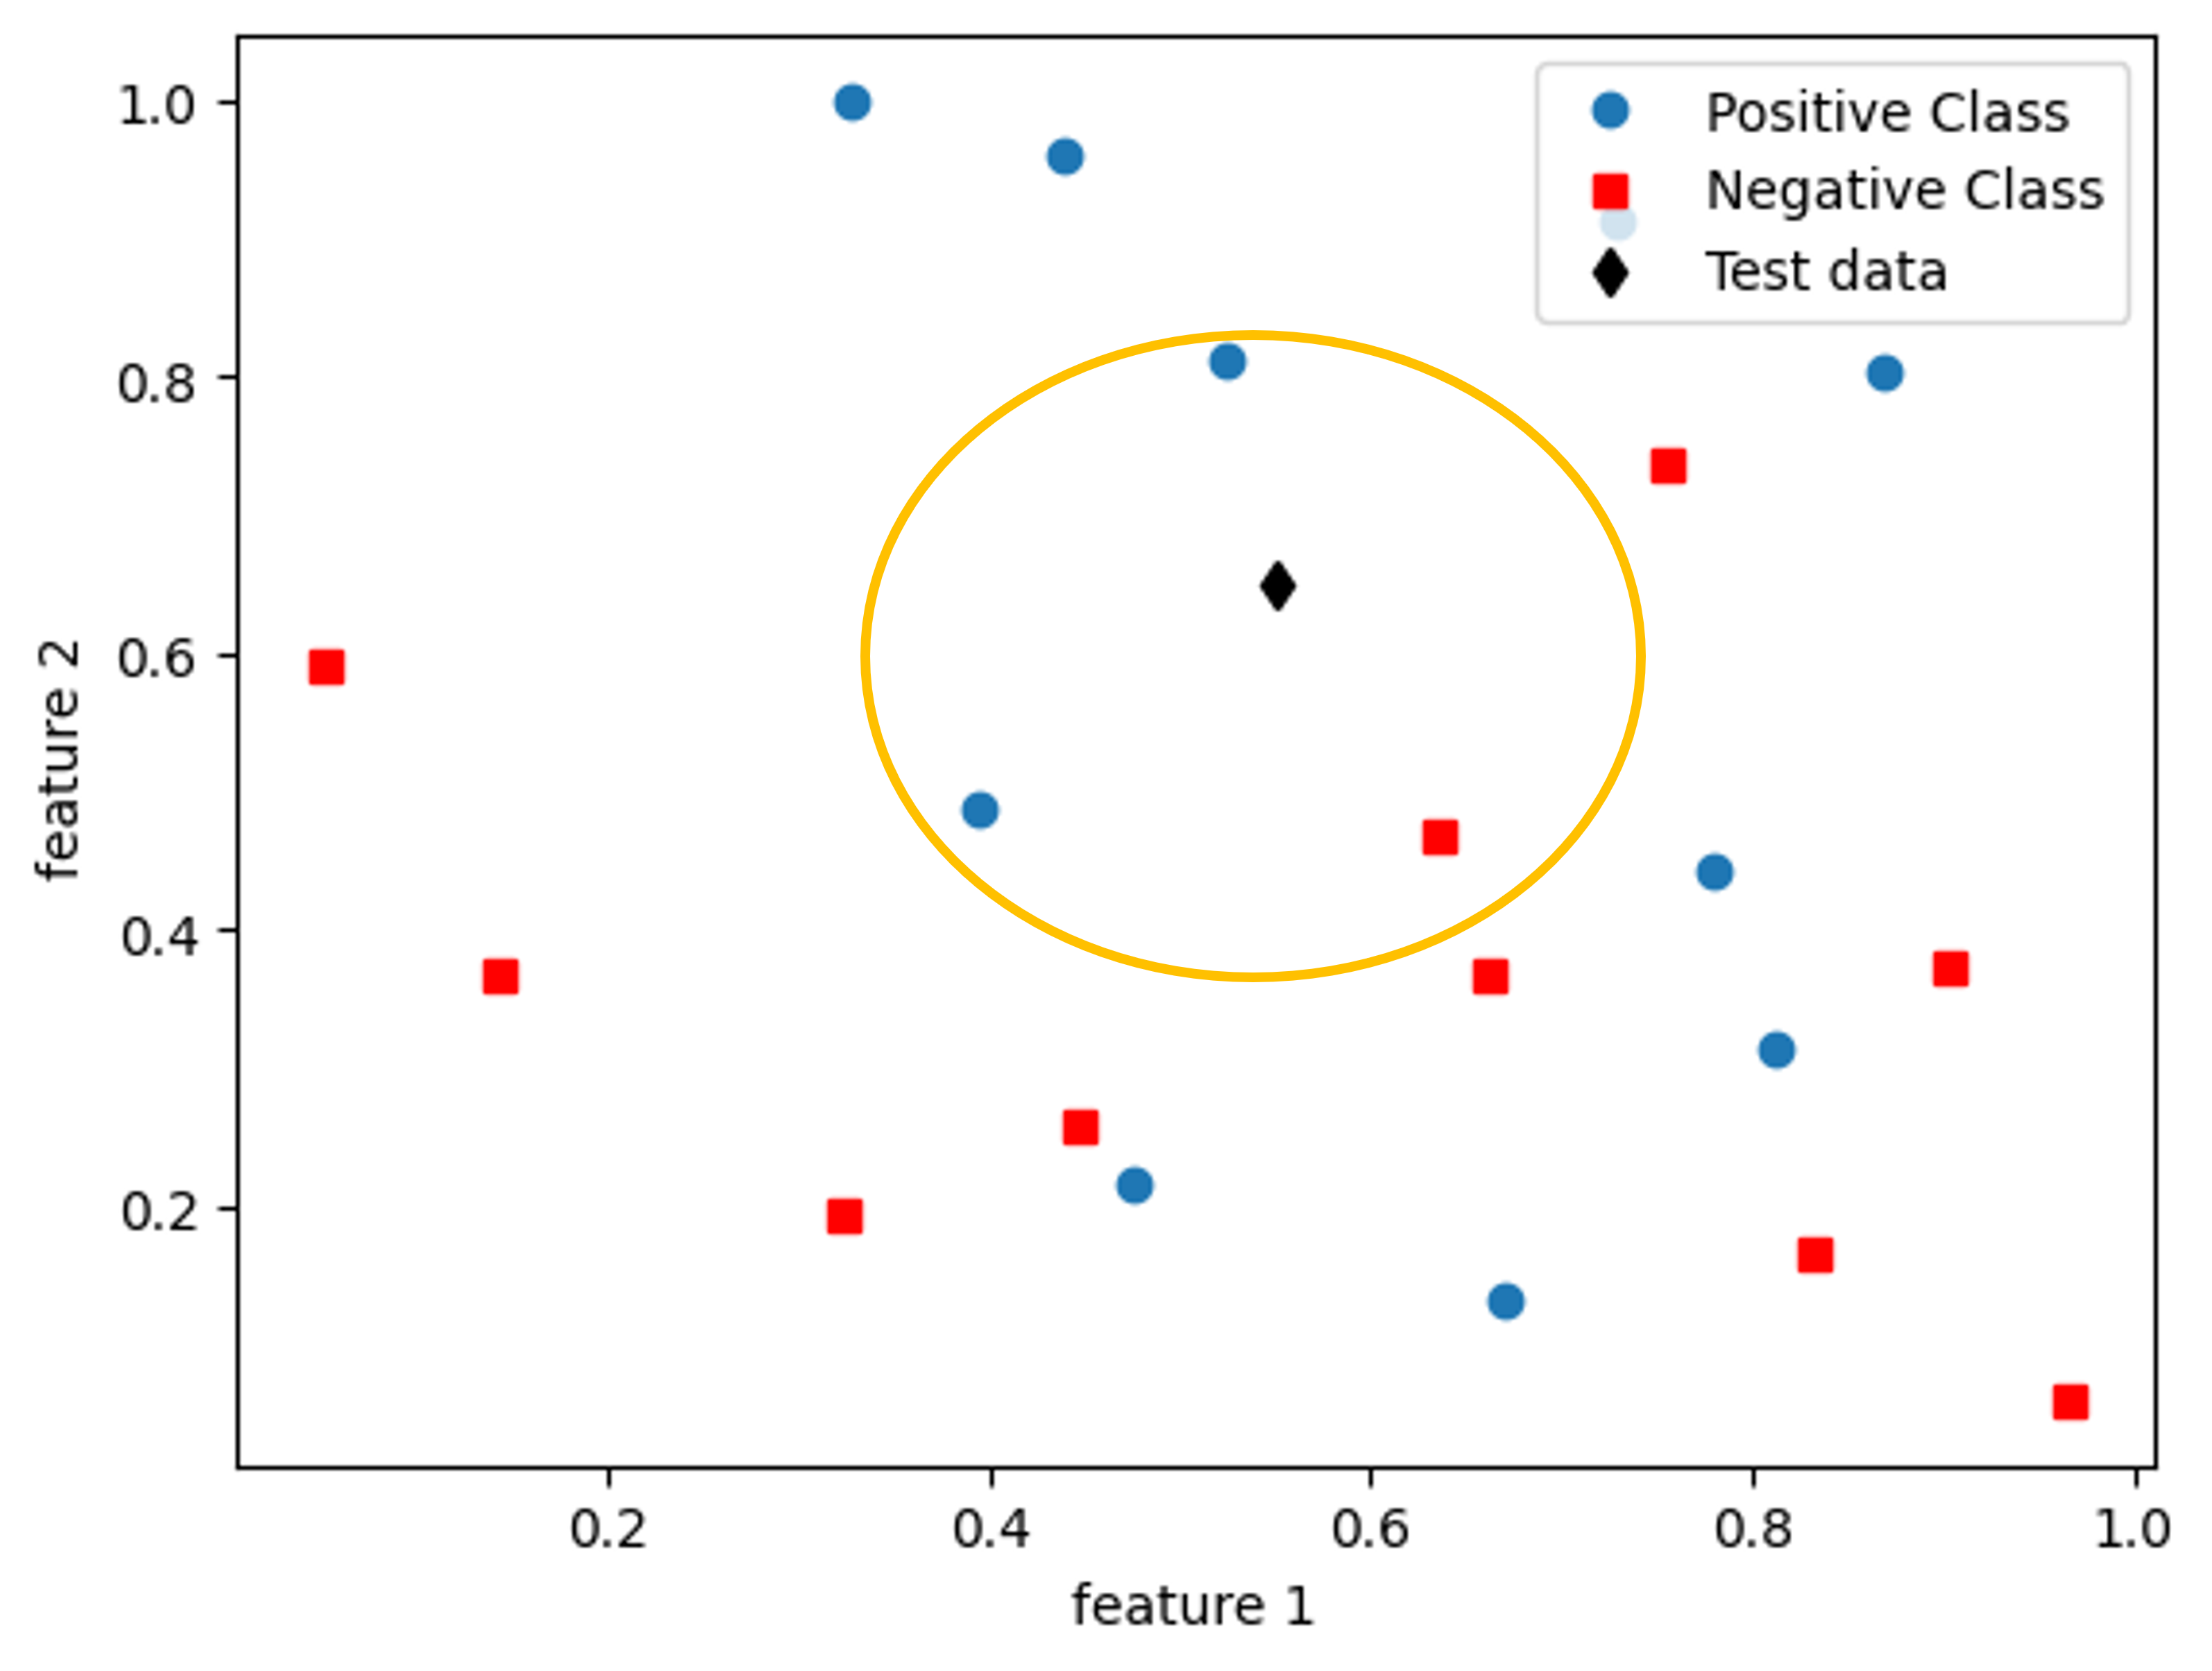
\includegraphics[width=7.5 cm]{knn_2.png}
  \caption{Concept of KNN}
  \label{fig:knn}
\end{figure}

The concept of k-NN is illustrated in Figure \ref{fig:knn}, using a simple example of a binary classification problem. The k-NN algorithm computes the distance between the new data point (represented by a black diamond) and all the data points in both the positive class (represented by blue circles) and the negative class (represented by red squares). In this example, the number of nearest neighbors is set to 3 (k = 3), as indicated by the yellow circle. In this case, two of the nearest neighbors of the test data belong to the positive class, and only one belongs to the negative class. As a result, the new data point will be assigned to the positive class.



\subsection{Distance Metrics in k-NN}
The initial step in k-NN is to calculate the distance from the new data point to all the other data points in the training data-set. One commonly used metric is the \textbf{Euclidean distance}, which measures the distance between two data points ($X_1$ and $X_2$) in an n-dimensional space. This distance is defined as:
\begin{equation}\label{eqn:eud}
  d(X_1, X_2) = \sum_{i=1}^n \sqrt{(x_1^i-x_2^i)^2}
\end{equation}

Another popular metric used in k-NN is the\textbf{ Manhattan distance}, which calculates the absolute distance between two data points and is defined as:

\begin{equation}\label{eqn:mah}
  d(X_1, X_2) = \sum_{i=1}^n \| x_1^i- x_2^i \|
\end{equation}

Other types of distance measures include Minkowski distance, cosine similarity, and Hamming distance.

\newpage
\subsection{Values of k in k-NN}
Another important parameter in the k-Nearest Neighbors (k-NN) method is the value of k, which represents the number of nearest neighbors that will be used to classify new data points. The choice of k can have a significant impact on the model's performance. A small value of k may result in a model that performs well on the training data set, but has high variance, meaning it may not generalize well to new, unseen data. On the other hand, a larger value of k may lead to a model with lower variance but higher bias, meaning it may not fit the training data as well.

\subsection{K-NN in Python}

The sample code below demonstrates how to implement the k-NN algorithm using Python.

\begin{lstlisting}
# ==================================================#
#--------------------------------------------------
## Using piepline to implement k-nn classifier ##
#--------------------------------------------------
from sklearn.neighbors import KNeighborsClassifier

steps = [('scaler', StandardScaler()),
         ('knn', KNeighborsClassifier(n_neighbors = 5))]
knn_pipeline = Pipeline(steps)
knn_pipeline.fit(X_train, y_train)
#--------------------------------------------------
## Model Evaluation ##
#--------------------------------------------------
from sklearn.metrics import classification_report
from sklearn.metrics import confusion_matrix
from sklearn.metrics import roc_auc_score


ypred_test = knn_pipeline.predict(X_test)
mat_clf = confusion_matrix(y_test, ypred_test)
report_clf = classification_report(y_test, ypred_test)

print(mat_clf)
print(report_clf)

ypred_testP = knn_pipeline.predict_proba(X_test)
auc = roc_auc_score(y_test, ypred_testP[:,1])
print(auc)
# ==================================================#
\end{lstlisting}

\newpage
\section{Support Vector Machine}
Support Vector Machine (SVMs) is a popular method for solving classification problems due to their strong performance. The goal of an SVM is to find a decision boundary that clearly separates different classes of data points.

In order to understand SVMs, it is important to be familiar with several key concepts, including: hyperplane, decision boundary, support vectors, margin, and SVM kernel.

\subsection{Hyperplane}
A hyperplane in geometry is a subspace of a vector space that has one dimension less than the vector space. For example, in a 2-dimensional vector space, a hyperplane is a line and in a 3-dimensional vector space, a hyperplane is a 2-dimensional plane (surface).

\subsection{Decision boundary}
A decision boundary is a line or \textbf{hyperplane} that divides different classes of data in a feature space, where a line is used in 2-dimensional space and a hyperplane is used in N-dimensional space, with N being the number of features.

Figure \ref{fig:svmEg} illustrates how decision boundaries can differ in 2-dimensional and 3-dimensional feature space. In 2D space, where there are only two features, classes can be separated by a straight line. However, in 3D space, the decision boundary becomes a plane. It can be difficult to envision in higher dimensional space, but most classification problems occur in higher dimensional space. Therefore, the SVM community typically refers to the decision boundary as a hyperplane in general. As demonstrated in Figure \ref{fig:svmEg}, more than one hyperplane can be used to separate the data into different classes.

\begin{figure}[!h]
  \centering
  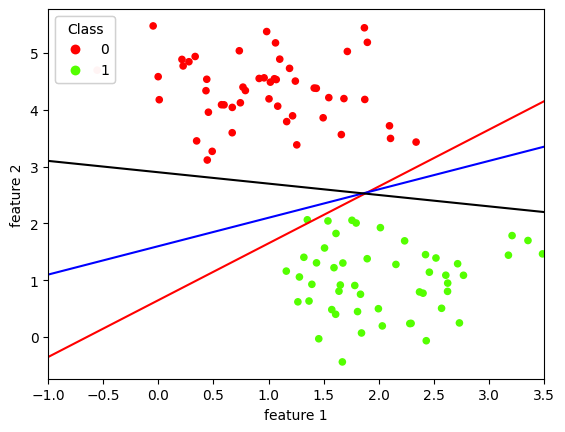
\includegraphics[width=4 cm]{svm_eg.png}
  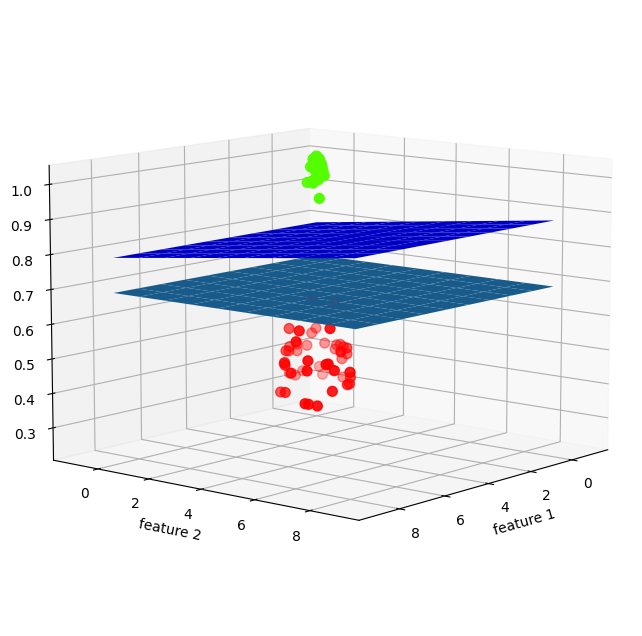
\includegraphics[width=4 cm]{svm_eg3d.png}
  \caption{Demonstration of SVM decision boundaries}
  \label{fig:svmEg}
\end{figure}

\subsection{Support Vectors}

SVM finds the hyperplane that separates the data points clearly by maximizing the gap between the decision boundary and the data points closest to it. These specific data points are known as "\textbf{support vectors}" in SVM.

\begin{figure}[!h]
  \centering
  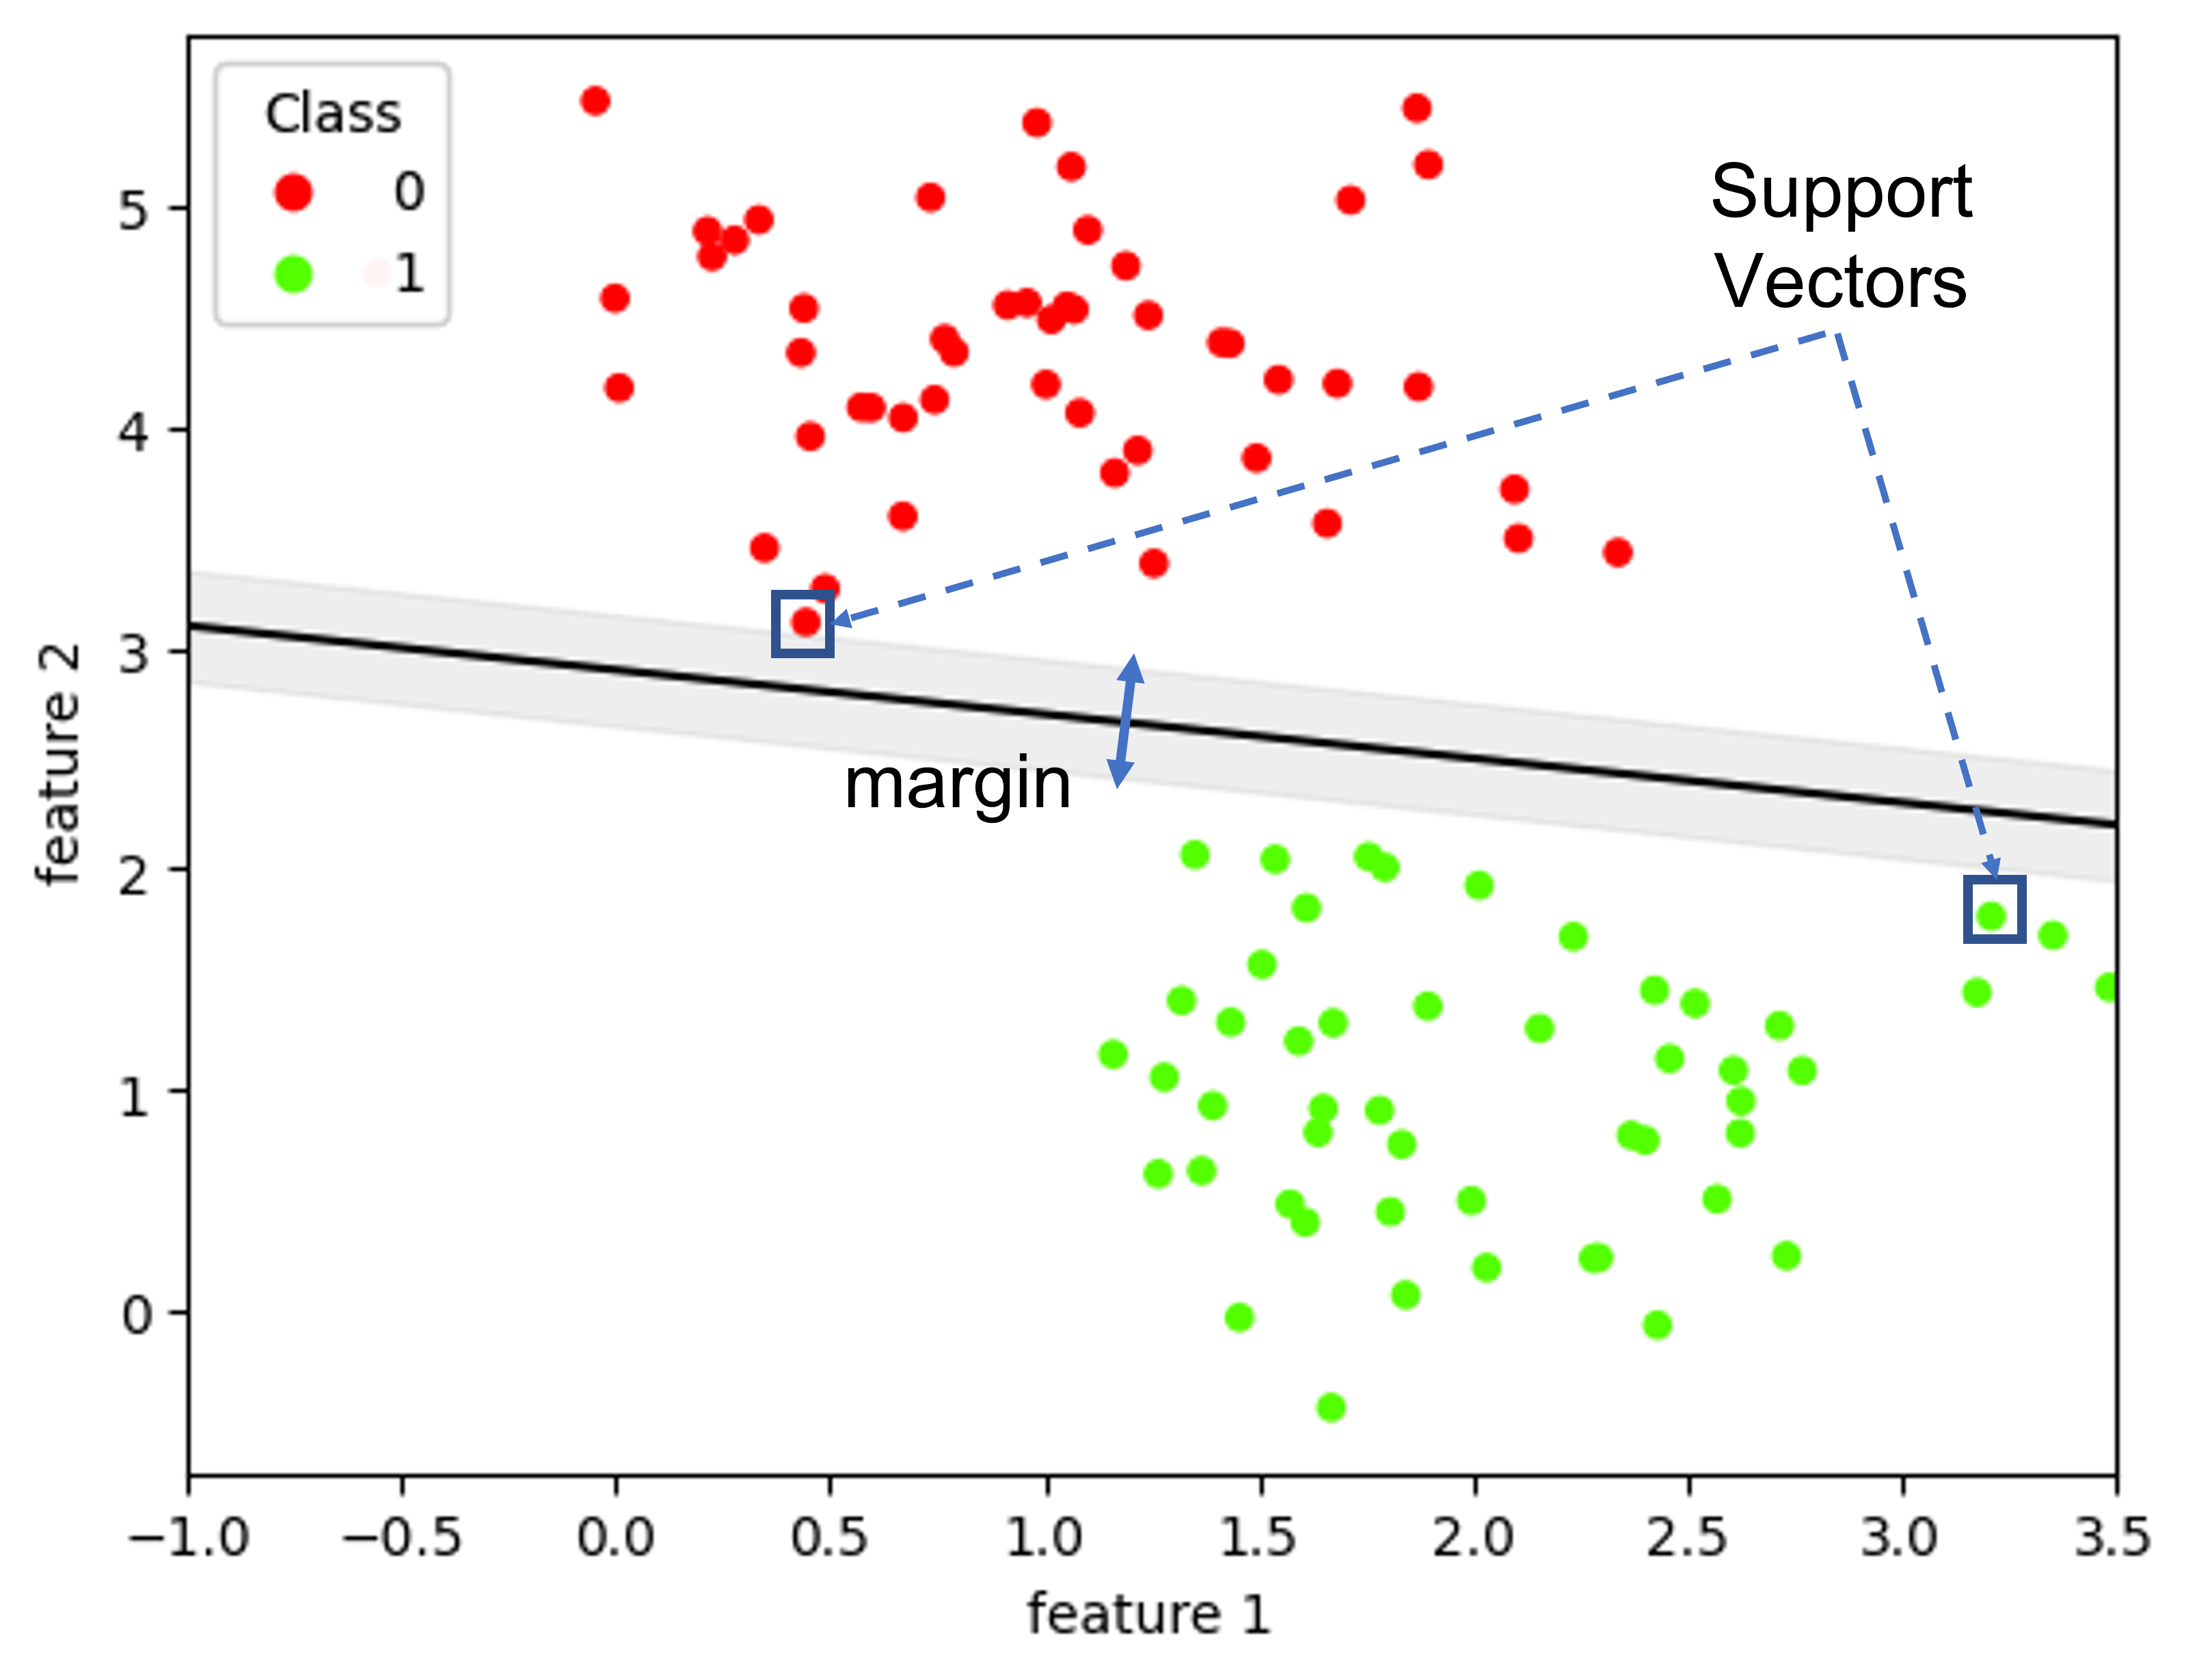
\includegraphics[width=8.0 cm]{svm_sv.png}
  \caption{Support Vectors in 2-Dimensional feature space}
  \label{fig:svm_SV}
\end{figure}

In Figure \ref{fig:svm_SV}, the support vectors are shown in the square box and removing these data points can alter the position and the orientation of the decision boundary.


%Hyperplane and decision boundary are equivalent at small dimension space, 'plane' has the meaning of straight and flat, so it is a line or a plane that separate the data sets. When you do a non-linear operation to map your data to a new feature space, the decision boundary is still a hyperplane in that space, but is not a plane any more at the original space.

%In the previous sections, we have learnt that logistic regression method finds a decision boundary (a line in 2-dimensional space) that minimizes the error between the predicted values and actual values. In other words, it maximizes the distance between the decision boundary and the data points. All the data points are considered in computing the distance.
%
%Similar to a linear regression/ logistic regression,  SVM maximizes the margin that has the maximum distance between the decision boundary and data points from both classes. SVM, instead of considering all data points like the linear regression, considers only the data points that are the closet to the decision boundary.

\subsection{Margin}
In SVM, the margin is the distance between the support vectors and the hyperplane, which is perpendicular. The goal of SVM is to find the maximum margin that can divide the data points between two classes. The margin is represented by the gray color in Figure \ref{fig:svm_SV}.

\subsection{SVM Kernels}
The data points shown in Figure \ref{fig:svm_SV} can be separated by a linear boundary, and SVM can identify the optimal hyperplane to distinguish between the two classes. However, in most real-world situations, the data points from different classes cannot be separated by a linear boundary. Figure \ref{fig:svm_K} shows an example of data points from two classes that cannot be separated by a linear boundary. One of the key advantages of SVM is its ability to use a kernel to classify non-linearly separable classes.

The role of a kernel is to change the data into a higher-dimensional space, making it possible for a hyperplane to distinguish different classes. There are various types of SVM-Kernels, and this section discusses three of them.

\begin{figure}[!h]
  \centering
  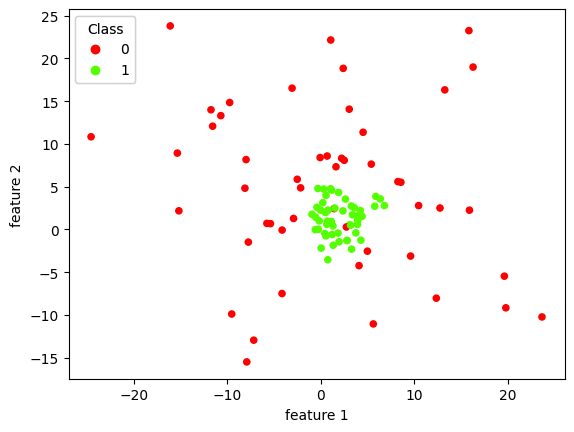
\includegraphics[width=8 cm]{svm_kernel.png}
  \caption{Linearly non-separable data set}
  \label{fig:svm_K}
\end{figure}

\newpage
\subsubsection{\textbf{Linear Kernel}}
A linear kernel is defined as:

\begin{equation}\label{eq:lin_kernel}
  K(X_1, X_2) = X_1^T X_2
\end{equation}This kernel is used only when the classes can be separated linearly.

\subsubsection{\textbf{Polynomial Kernel}}
A polynomial kernel utilizes a polynomial function to transform the data into a higher-dimensional space. The mathematical representation of this function is:

\begin{equation}\label{eq:poly_kernel}
  K(X_1, X_2) = (X_1^T X_2 + c)^d
\end{equation} where $c$ is the constant parameter and usually set at 0 or 1. $d$ is the degree (or order) of the polynomial function and $X_1$ and $X_2$ are n-dimensional data points.

Like polynomial regression, the degree $d$ is a hyper-parameter that controls the complexity of the kernel. The value of $d$ determines the degree of the polynomial function used to map the data into a higher-dimensional space. A higher degree of d means a more complex function, resulting in a more complex decision boundary, which can lead to over-fitting if the model is too complex for the data at hand.

On the other hand, a lower degree of $d$ means a simpler function and a simpler decision boundary, which can lead to under-fitting if the model is not complex enough to capture the underlying patterns in the data. Therefore, it is crucial to choose the appropriate degree d that balances the bias-variance trade-off as discussed in Section \ref{sec:hyperP}.


\subsubsection{\textbf{Radial Bias Function (RBF) kernel}}
RBF kernel computes the similarity between two data points $X_1$ and $X_2$ as follows:

\begin{equation}\label{eq:rbf}
  K(X_1, X_2) = \exp(-\gamma\|X_1-X_2\|^2)
\end{equation} where

\begin{equation}\label{eq:gamma}
  \gamma = \frac{1}{2\sigma^2}
\end{equation}and $\sigma$ is the variance of the kernel and control the width of the similarity region. $\|X_1-X_2\|$ is Euclidean ($L_2$-norm) distance between two data points $X_1$ and $X_2$.

\begin{figure}[!h]
  \centering
  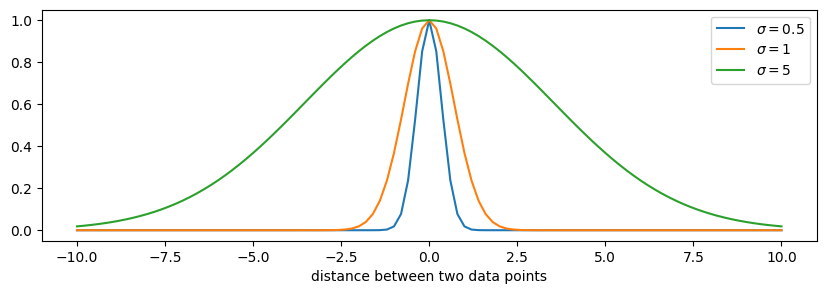
\includegraphics[width=8 cm]{kernel_dist.png}
  \caption{RBF kernel for different $\sigma$ values}
  \label{fig:kernel_d}
\end{figure}

The value of $\sigma$ decides which points should be considered as similar. Figure \ref{fig:kernel_d} illustrates how the $\sigma$ influences the region of the similarity. When the distance between two data points $\|X_1-X_2\|$ is zero, the value of the RBF kernel will always be one, regardless of the value of $\sigma$. Otherwise, the value of $\sigma$ affects the rate at which the RBF kernel decreases as the distance between two data points $\|X_1-X_2\|$  increases. When $\sigma$ is set to a low value, the RBF kernel decreases quickly, and when $\sigma$ is set to a high value, the RBF kernel decreases slowly. For example:

\begin{description}
  \item[case 1: $\sigma=0.5$] the value of the RBF kernel is zero when the distance is greater than 2.
  \item[case 2: $\sigma=1$] the value of the RBF kernel is zero when the distance is greater than 4.
  \item[case 3: $\sigma=5$] the value of the RBF kernel is zero only when the distance is greater than 10.
\end{description}


It is important to choose the appropriate value of $\sigma$ that balances the trade-off between over-fitting and under-fitting. A smaller value of $\sigma$ or a larger value of $\gamma$ may lead to over-fitting, as it only considers data points to be close if the distance between them is very small. The choice of the right value of the hyper-parameter $\gamma$ will significantly impact the performance of the RBF-SVM classifier.

\subsection{Hyper-parameters}

Hyper-parameter optimization plays a vital role in determining the performance of the SVM classifier. The key hyper-parameters that need to be considered are:

\subsubsection{\textbf{Kernel}}
The type of kernel is one of the hyper-parameters in implementing the SVM classifier, and the right choice of the kernel will lead to good performance. In Python, the grid or random search method can be used to find the right kernel.

\subsubsection{\textbf{Regularization parameter (C)}}
As discussed in Section \ref{sec:regularization}, a regularization term can be added to prevent the over-fitting and the parameter $C$ in Python sklearn controls the strength of the regularization. \href{https://www.csie.ntu.edu.tw/~cjlin/papers/guide/guide.pdf}{A practical guide to Support Vector Classifier} \cite{svmGuide:1984} guided that the value of the $C$ should be searched in the range of $C \in [2^{-5}, 2^15]$.

\subsubsection{\textbf{Degree (d)}}
In a polynomial kernel, the degree or order of the polynomial function is a hyper-parameter that needs to be tuned for the SVM classifier. Generally, the value of $d$ is set between 0 and 10.

\subsubsection{\textbf{Kernel coefficient ($\gamma$)}}
In RBF kernel, the value of $\gamma$ is an important hyper-parameter that needs to be selected. \href{https://www.csie.ntu.edu.tw/~cjlin/papers/guide/guide.pdf}{A practical guide to Support Vector Classifier} \cite{svmGuide:1984} guided the value of $\gamma$ should be searched within a range of $\gamma \in [2^{-15}, 2^3]$ to achieve optimal performance.

\newpage
\subsection{Linear SVM in Python}
The following code demonstrates how to implement a linear SVM classifier using the Python sklearn library.

\begin{lstlisting}
# ==================================================#
#--------------------------------------------------
## Using piepline to implement SVM classifier ##
#--------------------------------------------------
from sklearn.svm import SVC

steps = [('scaler', StandardScaler()),
         ('svc', SVC(kernel = 'linear'))]

svc_pipeline = Pipeline(steps)
svc_pipeline.fit(X_train, y_train)

#--------------------------------------------------
## Model Evaluation ##
#--------------------------------------------------
from sklearn.metrics import classification_report
from sklearn.metrics import confusion_matrix
from sklearn.metrics import roc_auc_score

ypred_test = svc_pipeline.predict(X_test)

mat_clf = confusion_matrix(y_test, ypred_test)
report_clf = classification_report(y_test, ypred_test)
auc = roc_auc_score(y_test, ypred_test)

# ==================================================#
\end{lstlisting}


\newpage
\subsection{Polynomial Kernel SVM in Python}

This section illustrates how to implement a non-linear SVM classifier using the polynomial kernel. The degree value $d$ is set at 5 in the SVC function. This hyper-parameter value can be adjusted using the ‘GridSearchCV’ method. The code for using the ‘GridSearchCV’ can be found in Section \ref{sec:hyperP}

\begin{lstlisting}
# ==================================================#
#--------------------------------------------------
## Using piepline to implement SVM Poly classifier ##
#--------------------------------------------------
from sklearn.svm import SVC

steps = [('scaler', StandardScaler()),
         ('svc', SVC(kernel = 'poly', degree = 5))]

svc_pipeline = Pipeline(steps)
svc_pipeline.fit(X_train, y_train)

#--------------------------------------------------
## Model Evaluation ##
#--------------------------------------------------
from sklearn.metrics import classification_report
from sklearn.metrics import confusion_matrix
from sklearn.metrics import roc_auc_score

ypred_test = svc_pipeline.predict(X_test)

mat_clf = confusion_matrix(y_test, ypred_test)
report_clf = classification_report(y_test, ypred_test)
auc = roc_auc_score(y_test, ypred_test)
# ==================================================#
\end{lstlisting}

\newpage
\subsection{RBF Kernel SVM in Python}
The following code demonstrates how to implement the RBF kernel using Python. The gamma value is set to $\gamma = \frac{1}{N\sigma_X}$ which is defined as a default value in the Python sklearn library and referred to as `scale'.
\begin{lstlisting}
# ==================================================#
#--------------------------------------------------
## Using piepline to implement SVM RBF classifier ##
#--------------------------------------------------
from sklearn.svm import SVC

steps = [('scaler', StandardScaler()),
         ('svc', SVC(kernel = 'rbf', gamma = 'scale'))]

svc_pipeline = Pipeline(steps)
svc_pipeline.fit(X_train, y_train)

#--------------------------------------------------
## Model Evaluation ##
#--------------------------------------------------
from sklearn.metrics import classification_report
from sklearn.metrics import confusion_matrix
from sklearn.metrics import roc_auc_score

ypred_test = svc_pipeline.predict(X_test)

mat_clf = confusion_matrix(y_test, ypred_test)
report_clf = classification_report(y_test, ypred_test)
auc = roc_auc_score(y_test, ypred_test)
# ==================================================#
\end{lstlisting}

%\section{Naïve Bayes’ Classifier}
%A Naïve Bayes’ Classifier is a probabilistic machine learning method that is based on the Bayes’ theorem.
%
%In Bayes’ theory, the probability for the output $y$ (a class label) is given by.
%Byaes theorem states that p(y j x) describes the
%probability for the output y (a class label) given that we know the input x.
%\subsection{Bernoulli Naive Bayes}
%\subsection{Multinomial Naive Bayes}
%\subsection{Gaussian Naive Bayes}
%\subsection{Implementation in Python}

\newpage
\section{Project: Fraud Detection}\label{sec:cls_proj1}
There are many other types of classifiers such as Naive Bayes classifier, tree-based classifiers, random forest, and deep learning methods that are not covered in this book. Deep learning methods have been extensively used in many research publications.

However, many researchers and practitioners have pointed out that the choice of a machine learning method depends on various factors, including the specific problem, the size and complexity of the data-set, and the computational resources available.

In this section, we will present the full codes for fraud detection using Logistic Regression, K-NN, and SVM classifiers. We will also compare the performance of these classifiers using the 'accuracy' and 'recall' metrics discussed in Section \ref{sec:Clsevaluation}.

The data-set \cite{web:fraudData} used in this analysis contains $21,693$ entries and $29$ independent features. This data-set is imbalanced, with $21,337$ non-fraud cases and $356$ fraud cases. The data is already cleaned and there is no missing data. The data-set can be downloaded from \href{https://github.com/yonycherkos/Applied-Data-Science-with-Python-Specialization.git}{the link provided} \cite{web:fraudData}.

\newpage
\subsection{Data Importing}
The first step is to import the necessary modules and import the data from the computer.

\begin{lstlisting}
# ==================================================#
import pandas as pd

df=pd.read_csv('..\\data\\fraud.csv', index_col = 0)
y = df['Class'].values
df = df.iloc[:,1:]
X = df.drop(columns = 'Class').values
# ==================================================#
\end{lstlisting}

\subsection{Splitting the data}

The next step is to divide the data into a training dataset and a testing dataset. 60\% of the data is allocated for training and the remaining 40\% is reserved for testing.

\begin{lstlisting}
# ==================================================#
from sklearn.model_selection import train_test_split

X_train, X_test, y_train, y_test = train_test_split(X,y,
                                    test_size = 0.40,
                                    random_state=1)
# ==================================================#
\end{lstlisting}

\subsection{Modelling}
Five different classifiers are developed. The names and hyper-parameters of the classifiers are provided in Table \ref{tb:clf_parameters}.
Regularization is added to all classifiers, except K-NN and the strength of regularization is controlled by the parameter $C$. In logistic regression, the $L2$ term is used for regularization and squared $L2$ is used for SVM classifiers.

The number of neighbors in K-NN is controlled by the value of $k$ and the order or degree of the polynomial function in SVM is defined as $3$. The kernel coefficient $\gamma$ for SVM-RBF kernel is defined as $\gamma = \frac{1}{N\sigma_{Xtr}}$.

\begin{table}[!ht]
\centering
\begin{tabular}{|c|c|c| }
  \hline
  Name & \multicolumn{2}{|c|}{Hyper-parameters}\\
  \hline
  LR  & C = 1.0& \\
  \hline
  KNN & k = 5  & \\
  \hline
  SVM-Linear & C = 1.0 &   \\
  \hline
  SVM-Poly &  C = 1.0  &  degree = 3\\
  \hline
  SVM-RBF & C = 1.0    & $\gamma = \frac{1}{N\sigma_{Xtr}}$\\
  \hline
\end{tabular}
\caption{Classifier model and its hyper-parameters}\label{tb:clf_parameters}
\end{table}

\newpage
\begin{lstlisting}
# ==================================================#
from sklearn.preprocessing import StandardScaler
from sklearn.pipeline import Pipeline
#--------------------------------------------------
## ------------Logistic Regression----------------##
#--------------------------------------------------

from sklearn.linear_model import LogisticRegression

steps = [('scaler', StandardScaler()),
         ('logReg', LogisticRegression(penalty = "l2",
                                        C = 1.0))]

LR_pipeline = Pipeline(steps)
LR_pipeline.fit(X_train, y_train)
#--------------------------------------------------
## ----------- K-NN Classifier ------------------##
#--------------------------------------------------

from sklearn.neighbors import KNeighborsClassifier

steps = [('scaler', StandardScaler()),
         ('knn', KNeighborsClassifier(n_neighbors = 5))]

knn_pipeline = Pipeline(steps)
knn_pipeline.fit(X_train, y_train)
#--------------------------------------------------
## ------------ SVM Classifier ------------------##
#--------------------------------------------------
from sklearn.svm import SVC
## Linear Kernel  ---------------
steps = [('scaler', StandardScaler()),
         ('svc', SVC(kernel = 'linear',
                     class_weight='balanced'))]

svcL_pipeline = Pipeline(steps)
svcL_pipeline.fit(X_train, y_train)
## Polynomial Kernel -----------------------
steps = [('scaler', StandardScaler()),
         ('svc', SVC(kernel = 'poly', degree = 3,
                     class_weight='balanced'))]

svcPoly_pipeline = Pipeline(steps)
svcPoly_pipeline.fit(X_train, y_train)
## RBF Kernel -----------------------
steps = [('scaler', StandardScaler()),
         ('svc', SVC(kernel = 'rbf', gamma = 'scale',
                     class_weight='balanced'))]

svcRBF_pipeline = Pipeline(steps)
svcRBF_pipeline.fit(X_train, y_train)
# ==================================================#
\end{lstlisting}

\subsection{Model Evaluation}
The classifiers are evaluated using three metrics: 'accuracy', 'recall', and 'area under the curve'. As discussed in Section \ref{sec:Clsevaluation}, 'recall' is an essential metric for fraud detection as we do not want to miss any fraud case. It is better to have false alarms than missing a fraud. The following codes calculate the metrics using the \emph{classification report function} under sklearn.metrics module  and extract the accuracy and recall parameters. The function roc\-auc\_score is used to compute the area under the curve. The evaluation is done for both the training and testing sets, and the results are saved in a tabular format.

\begin{lstlisting}
# ==================================================#
from sklearn.metrics import classification_report
from sklearn.metrics import roc_auc_score

result_df = pd.DataFrame(columns = ['Tr_accuracy',
                                    'Test_accuracy',
                                    'Tr_recall',
                                    'Test_recall',
                                    'Train_auc',
                                    'Test_auc'])

model_name = [LR_pipeline, knn_pipeline, svcL_pipeline,
              svcPoly_pipeline, svcRBF_pipeline]
for idx, model in enumerate(model_name):
    ## for training data
    ypred_train = model.predict(X_train)
    report_clf = classification_report(y_train,
                                       ypred_train,
                                       output_dict=True)
    df_r = pd.DataFrame(report_clf).transpose()
    acc_tr = df_r.loc['accuracy', 'recall'].round(3)
    recall_tr = df_r.iloc[1,1].round(3)
    auc_tr = roc_auc_score(y_train, ypred_train)
    ## for testing data
    ypred_test = model.predict(X_test)
    report_clf = classification_report(y_test,
                                       ypred_test,
                                       output_dict=True)
    df_r = pd.DataFrame(report_clf).transpose()
    acc = df_r.loc['accuracy', 'recall'].round(3)
    recall = df_r.iloc[1,1].round(3)
    auc = roc_auc_score(y_test, ypred_test)

    result_df.loc[idx,:]=[acc_tr, acc, recall_tr,
                          recall, auc_tr.round(3),
                          auc.round(3)]
result_df.index = ['LR', 'K-NN', 'SVM-Linear',
                   'SVM-Poly', 'SVM-RBF']
# ==================================================#
\end{lstlisting}

\subsection{Discussion on Performance}

\subsubsection{\textbf{Accuracy}}

Table \ref{tb:accR} lists the accuracy scores for different classifiers. The SVM-linear model performs the worst with an accuracy score of 97\%. The performance is similar for both the training and testing sets.

However, as discussed in Section \ref{tb:clf_parameters}, accuracy score is not a good measure for imbalanced classes. Our data-set has 98\% of non-fraud cases and only 2\% of fraud cases. This is a common scenario in many problems such as cancer detection, spam detection, etc. The negative class (class 0) always has more data than the positive class (class 1).

\begin{table}[!ht]
\centering
\csvreader[tabular=|c|r|r|, ,table head=\hline & Train & Test \\\hline, late after line=\\\hline]%
{data/accuracy.csv}{Name= \Name, Train=\Train, Test=\Test}{\Name & \Train & \Test}
\caption{Accuracy for Fraud Detection using different methods.}\label{tb:accR}
\end{table}

\subsubsection{\textbf{Recall}}

Table \ref{tb:accR} lists the recall values for different classifiers. The SVM with the RBF kernel performs the best with a score of 99\% for the training data-set. It means that 99\% of the fraud cases in the training set are successfully detected by the SVM-RBF classifier. However, it can be observed that the SVM-RBF over-fits the training data, and it performs the worst for the testing data-set. The SVM classifier with the linear model produces reasonable results for both the training and testing data-sets at 91\% and 88\% respectively. The SVM-linear classifier has a good balance between bias and variance.

\begin{table}[!ht]
\centering
\csvreader[tabular=|c|r|r|, ,table head=\hline & Train & Test \\\hline, late after line=\\\hline]%
{data/recall.csv}{Name= \Name, Train=\Train, Test=\Test}{\Name & \Train & \Test}
\caption{Recall for Fraud Detection using different methods.}\label{tb:recallR}
\end{table}

\subsubsection{\textbf{Area under the Curve}}
Table \ref{tb:accR} lists the areas under the curve for fraud detection using different classifiers. Similar to the recall score, the SVM classifier with the linear model produces the best results (94\% for training and 92.7\% for testing set) without over-fitting the problem.

\begin{table}[!ht]
\centering
\csvreader[tabular=|c|r|r|, ,table head=\hline & Train & Test \\\hline, late after line=\\\hline]%
{data/auc.csv}{Name= \Name, Train=\Train, Test=\Test}{\Name & \Train & \Test}
\caption{Area under the curve using different methods.}\label{tb:aucR}
\end{table}

The results from this project suggest that the complexity of the model does not always lead to better performance. Higher model complexity can cause over-fitting, leading to high variance in the results. Hyper-parameters can be adjusted to enhance the performance of the classifier.
